\section{UserRegisterComponent Klassenreferenz}
\label{classUserRegisterComponent}\index{UserRegisterComponent@{UserRegisterComponent}}
Klassendiagramm für UserRegisterComponent::\begin{figure}[H]
\begin{center}
\leavevmode
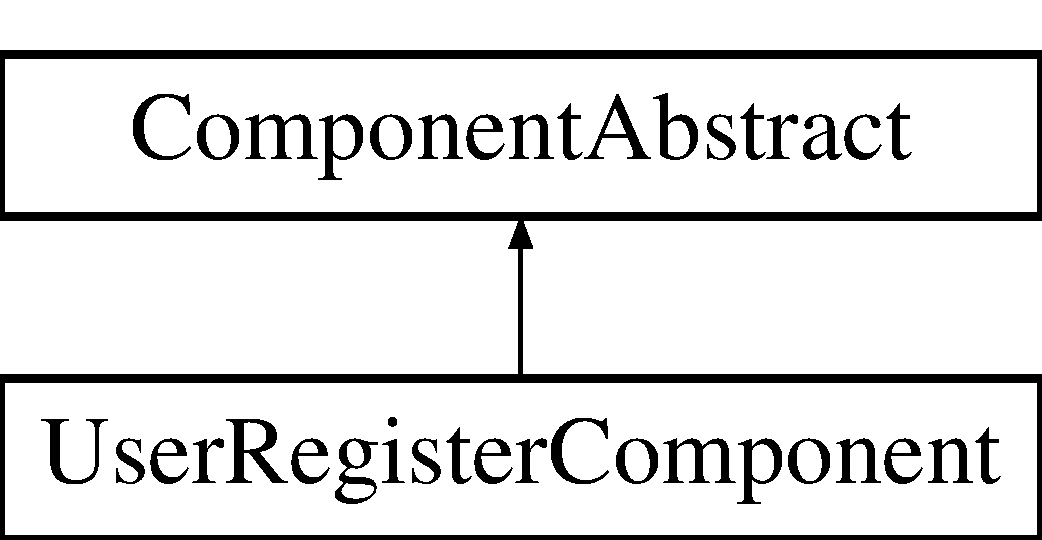
\includegraphics[height=2cm]{classUserRegisterComponent}
\end{center}
\end{figure}
\subsection*{Öffentliche Methoden}
\begin{CompactItemize}
\item 
{\bf UserRegisterComponent} (\$instanceID, \$instanceName, \&\$smartyObj)
\item 
{\bf redender} ()
\item 
{\bf getOutput} ()
\end{CompactItemize}


\subsection{Ausführliche Beschreibung}


Definiert in Zeile 9 der Datei UserRegisterComponent.php.

\subsection{Dokumentation der Elementfunktionen}
\index{UserRegisterComponent@{UserRegisterComponent}!UserRegisterComponent@{UserRegisterComponent}}
\index{UserRegisterComponent@{UserRegisterComponent}!UserRegisterComponent@{UserRegisterComponent}}
\subsubsection{\setlength{\rightskip}{0pt plus 5cm}UserRegisterComponent.UserRegisterComponent (\$ {\em instanceID}, \$ {\em instanceName}, \&\$ {\em smartyObj})}\label{classUserRegisterComponent_944dfff60cd110cf8f294c06468ad128}




Definiert in Zeile 11 der Datei UserRegisterComponent.php.\index{UserRegisterComponent@{UserRegisterComponent}!redender@{redender}}
\index{redender@{redender}!UserRegisterComponent@{UserRegisterComponent}}
\subsubsection{\setlength{\rightskip}{0pt plus 5cm}UserRegisterComponent.redender ()}\label{classUserRegisterComponent_de635d3e68bf646897b503ccf5dae7ab}


Redender component 

Definiert in Zeile 19 der Datei UserRegisterComponent.php.

Benutzt \$\_\-GET und ComponentAbstract.getComponentID().\index{UserRegisterComponent@{UserRegisterComponent}!getOutput@{getOutput}}
\index{getOutput@{getOutput}!UserRegisterComponent@{UserRegisterComponent}}
\subsubsection{\setlength{\rightskip}{0pt plus 5cm}UserRegisterComponent.getOutput ()}\label{classUserRegisterComponent_17cfa6f974893b73264b0e8b63f82721}


return string of redendered component

\begin{Desc}
\item[Rückgabe:]string \end{Desc}


Definiert in Zeile 103 der Datei UserRegisterComponent.php.

Die Dokumentation für diese Klasse wurde erzeugt aufgrund der Datei:\begin{CompactItemize}
\item 
{\bf UserRegisterComponent.php}\end{CompactItemize}
